\section{Results}\label{sec:pecanrtm-results}

\subsection{Validation}

\subsubsection{Reflectance and transmittance}

For the inversion of synthetic spectra, we found no statistically significant ($p < 0.05$) spectral bias at any wavelength (not shown).% (Figure S6). %TODO: Figure
As well, the observed differences between input and simulated output were one to two orders of magnitude smaller than corresponding errors in the inversion of measured spectra (Figure~\ref{fig:pecanrtm-specvalidation}).%, Figure S6). %TODO: Figure references
These results collectively illustrate that our algorithm is unbiased and contributes minimally to errors in the inversion of measured spectra.

For the inversion of measured spectra, we observed substantial variability in the spectral bias across all analyzed leaves, resulting in statistically significant ($p < 0.05$) bias in only a few specific wavelength regions (Figure~\ref{fig:pecanrtm-specvalidation}). % TODO: Figure ref
For both broadleaf and needle-leaf conifer species, reflectance was typically overestimated between 1600 and 1900 nm and underestimated between 1000 and 1300 nm and between 2000 and 2500 nm.
The errors in the 1600 to 1900 nm and 2000 to 2500 nm ranges covered more wavelengths and had larger magnitude for conifer species than broadleaved species.
Broadleaved species also had a statistically significant reflectance overestimate in the 400 to 500 nm range and an underestimate at 1300 nm, while conifer species had a significant reflectance overestimate at 1300 nm.

For both measured and synthetic spectra, transmittance bias ($BIAS = -0.0133$) was, on average, greater in magnitude than reflectance bias ($BIAS = 0.0018$), with a mean positive bias for broadleaved species ($BIAS = 0.0012$) and a mean negative bias for conifer species ($BIAS = -0.0346$) (Figure~\ref{fig:pecanrtm-specvalidation}, Table~\ref{tab:pecanrtm-specerr}).
However, the between-leaf variability in bias was also large and resulted in statistically significant bias in only a small number of specific spectral regions.
For both broadleaved and conifer species, we observed a significant underestimate in transmittance in the chlorophyll a absorption 400 and 500 nm.
Specifically for conifer species, we also observed underestimates in transmittance at the vegetation ``red edge'' around 700 nm and at a water absorption feature around 1900 nm.

\begin{figure}
  \centering
  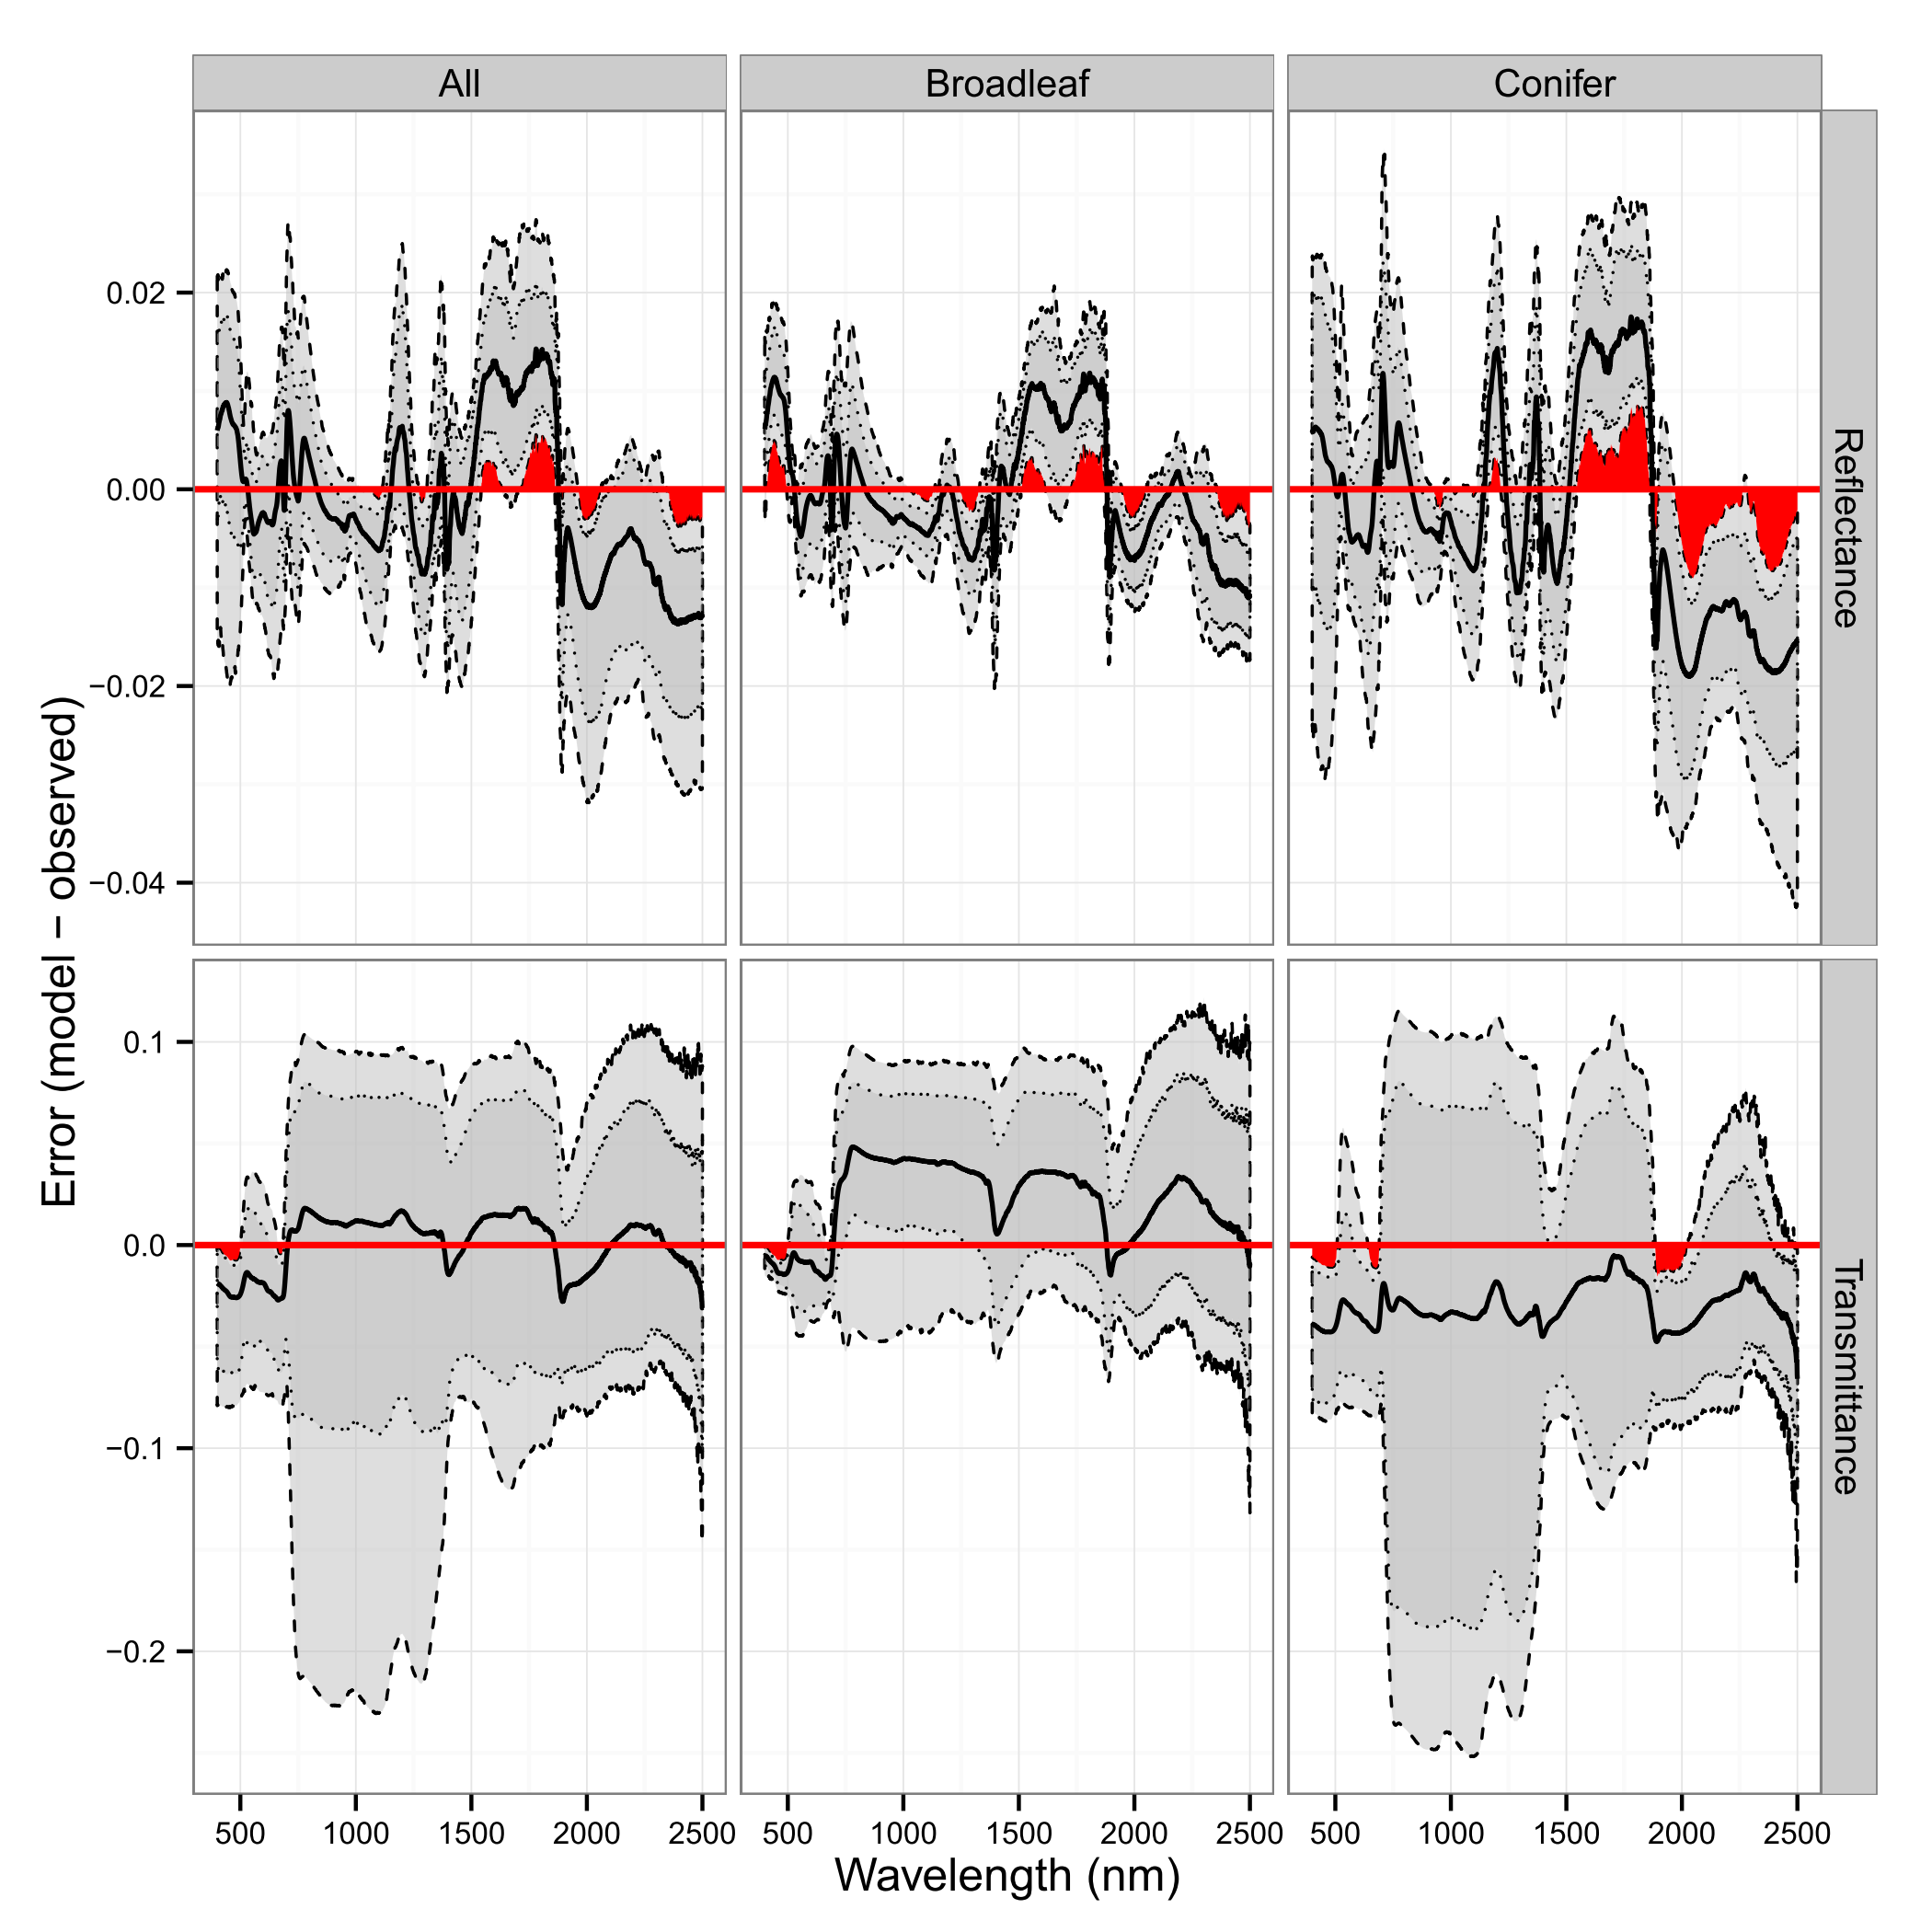
\includegraphics[width=\textwidth]{2_rtm_inversion/figures/spec_validation.png}
  \caption{%
    Bias in FFT simulated reflectance (top) and transmittance (bottom) spectra compared to measurements over all leaves (left) and only hardwood (middle) and conifer (right) species. 
    For a given wavelength,
    the solid black line is the mean bias,
    the dark grey bounded by the dotted line is the 90\% confidence interval,
    the light grey region bounded by the dashed line is the 95\% confidence interval,
    the red line highlights a bias of 0,
    and the red shaded regions highlight bias significant at the 95\% confidence level.
  }\label{fig:pecanrtm-specvalidation}
\end{figure}

\begin{table}
  \centering
  \caption{%
    Reflectance (Refl.) and transmittance (Tran.) spectral validation error statistics aggregated across the visible (400--800 nm) and infrared (801--2500 nm) regions.
    Values from other studies are included for comparison.
  }\label{tab:pecanrtm-specerr}
  \resizebox{\textwidth}{!}{%
    \begin{tabular}{clcccccc}
      \toprule
      & & \multicolumn{3}{c}{Visible} & \multicolumn{3}{c}{Infrared}\\
      & & RMSE & BIAS & SEPC & RMSE & BIAS & SEPC \\
      \midrule
      \multirow{7}{*}{Refl.} & FFT All & 0.0083 & 0.0018 & 0.0071 & 0.0098 & -0.0020 & 0.0061 \\
                             & --- Broadleaf & 0.0063 & 0.0023 & 0.0042 & 0.0064 & -0.0009 & 0.0034 \\
                             & --- Conifer & 0.0101 & 0.0011 & 0.0090 & 0.0127 & -0.0035 & 0.0064 \\
                             & Feret et al.~(2008): CALMIT & 0.032 & 0.010 & 0.028 & --- & --- & --- \\
                             & --- ANGERS & 0.019 & 0.001 & 0.019 & 0.016 & 0.003 & 0.014 \\
                             & --- HAWAII & 0.021 & -0.008 & 0.020 & 0.036 & -0.031 \\
                             & Di Vittorio (2009) & 0.0255 & 0.005 & --- & --- & --- & --- \\
      \midrule
      \multirow{7}{*}{Trans.} & FFT All & 0.0404 & -0.0133 & 0.0336 & 0.0551 & 0.0040 & 0.0537 \\
                              & --- Broadleaf & 0.0248 & 0.0012 & 0.0167 & 0.0450 & 0.0266 & 0.0336 \\
                              & --- Conifer & 0.0553 & -0.0346 & 0.0389 & 0.0661 & -0.0293 & 0.0566 \\
                              & Feret et al.~(2008): CALMIT & 0.029 & -0.005 & 0.025 & --- & --- & --- \\
                              & --- ANGERS & 0.018 & -0.005 & 0.017 & 0.016 & 0.001 & 0.015 \\
                              & --- HAWAII & 0.022 & 0.003 & 0.020 & 0.020 & -0.003 & 0.017 \\
                              & Di Vittorio (2009) & 0.0422 & 0.0294 & --- & --- & --- & --- \\
      \bottomrule
    \end{tabular}
  }
\end{table}

\begin{table}
  \centering
  \caption{%
    Error statistics for the comparison of inversion estimates of PROSPECT parameters Cw and Cm and measured values of equivalent water thickness (EWT) and leaf dry mass per unit area (LMA), respectively.
    Values from other inversion studies are included for comparison.
  }\label{tab:pecanrtm-paramerr}
  \begin{tabular}{p{2cm}lccccc}
    \toprule
    & & RMSE & BIAS & SEPC & CV & RMS\%E \\
    \midrule
    \multirow{7}{*}{\vtop{\hbox{Cw / EWT }\hbox{(g m$^{-2}$)}}}
    & FFT Broadleaf & 17 & 5 & 16 & 18.8 & 21.64 \\
    & --- Conifer & 187 & 90 & 164 & 52.3 & 67.29 \\
    & Feret et al.~(2008): LOPEX & 17 & -3 & 17 & 15.2 & --- \\
    & --- ANGERS & 20 & -1 & 20 & 17.1 & --- \\
    & Feret et al.~(2011): \#3 & 27 & --- & --- & --- & --- \\
    & Li \& Wang (2011) & 12 & 5 & --- & 20.10 & --- \\
    \midrule
    \multirow{7}{*}{\vtop{\hbox{Cm / LMA}\hbox{(g m$^{-2}$)}}}
    & FFT Broadleaf & 20 & -18 & 9 & 24.5 & 43.75 \\
    & --- Conifer & 121 & 35 & 116 & 61.6 & 65.51 \\
    & Feret et al.~(2008): LOPEX & 34 & 21 & 27 & 51.0 & --- \\
    & --- ANGERS & 26 & 1 & 26 & 49.8 & --- \\
    & Feret et al.~(2011): \#3 & 31 & --- & --- & --- & --- \\
    & Li \& Wang (2011) & 8 & -7 & --- & 13.75 & --- \\
    \bottomrule
  \end{tabular}
\end{table}

\subsubsection{Leaf water content and mass per area}

Similar to the results of the spectral validation,
the inversion estimates of Cw and Cm (compared to measured values of EWT and LMA, respectively) displayed higher accuracy for broadleaf ($CV_{Cw} = 18.8\%$, $CV_{Cm} = 24.5\%$) versus conifer species ($CV_{Cw} = 52.3\%$, $CV_{Cm} = 63.3\%$) (Table~\ref{tab:pecanrtm-paramerr}).
For the broadleaved species, our parameter estimates were within the range observed previously (Table~\ref{tab:pecanrtm-paramerr}).
While the inversion estimates for conifer species show a lower performance compared to broadleaf trees, the error inversion results were primarily driven by a single plant functional type—early successional conifers, which consisted entirely of pine species (\textit{Pinus} family).
Notably, a few estimates for mid-successional conifer species displayed significant divergence with observations, but in general fell along the 1:1 relationship (Figures~\ref{fig:pecanrtm-ewt} and~\ref{fig:pecanrtm-lma}).

\begin{figure}
  \centering
  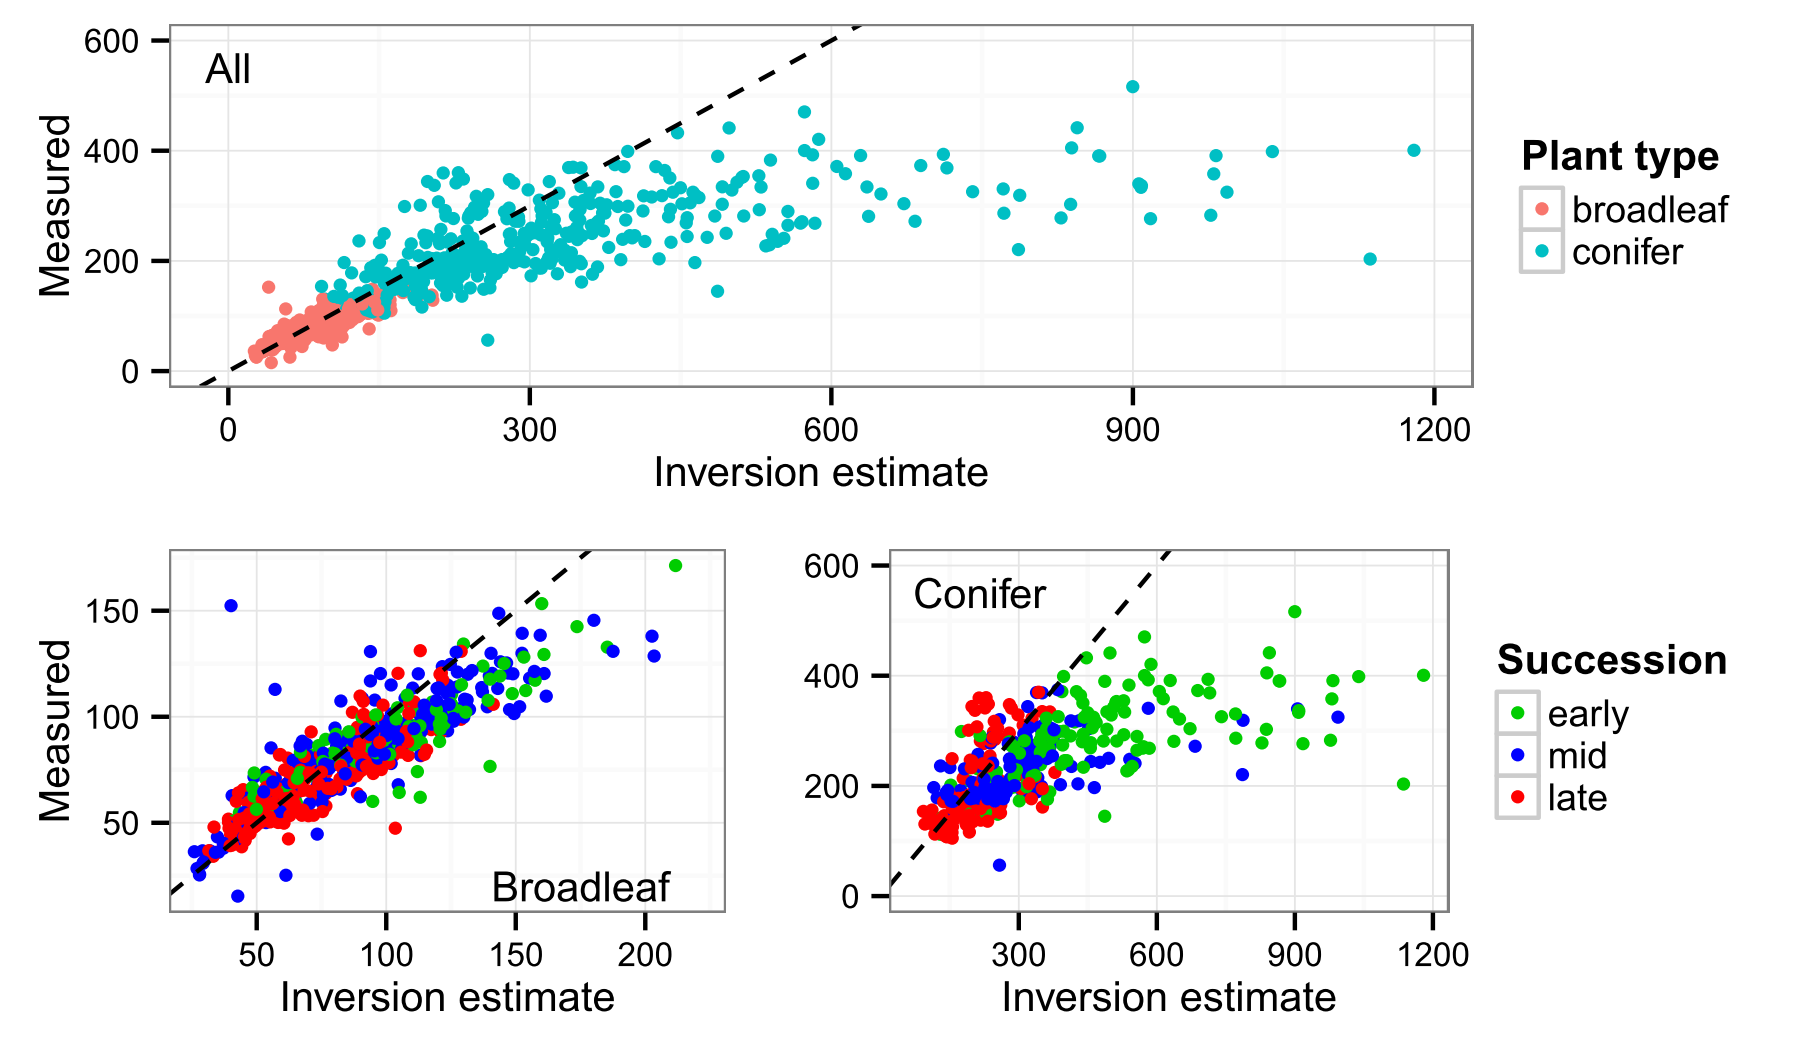
\includegraphics[width=\textwidth]{2_rtm_inversion/figures/ewt_validation.png}
  \caption{%
    Modeled and observed equivalent water thickness (g m$^{-2}$) for both conifers and hardwoods (top), just hardwoods (bottom left), and just conifers (bottom right).
    Point colors indicate plant type (top) or successional stage (bottom).
    The dashed line represents a 1:1 fit.
  }\label{fig:pecanrtm-ewt}
\end{figure}

\begin{figure}
  \centering
  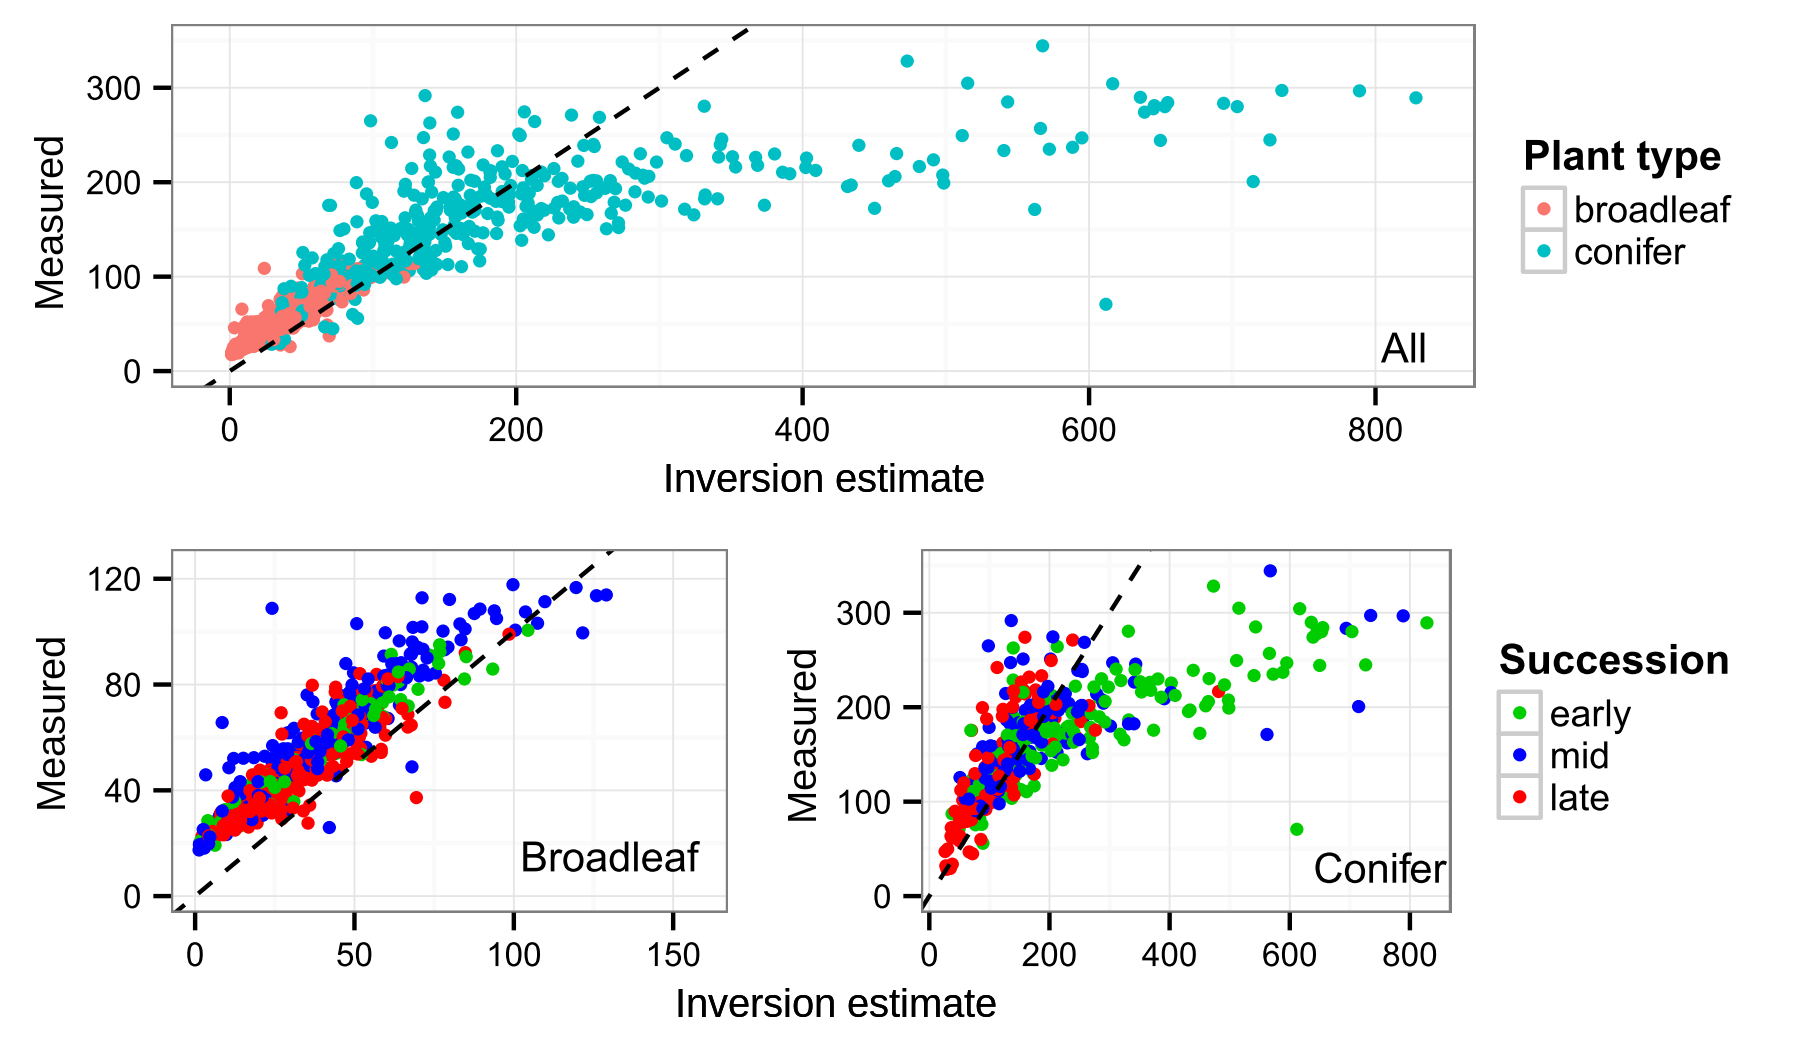
\includegraphics[width=\textwidth]{2_rtm_inversion/figures/lma_validation.png}
  \caption{%
    Modeled and observed leaf dry mass per unit area (g m$^{-2}$) for both conifers and hardwoods (top), just hardwoods (bottom left), and just conifers (bottom right).
    Point colors indicate plant type (top) or successional stage (bottom).
    The dashed line represents a 1:1 fit.
  }\label{fig:pecanrtm-lma}
\end{figure}

\subsection{Sensor simulation experiment}

\subsubsection{Parameter error}

\begin{table}
  \centering
  \caption{%
    Uncertainty and relative bias in parameter estimates from inversion of simulated spectra filtered through relative spectral response curves of different sensors.
  }\label{tab:pecanrtm-sensorerror}
  \resizebox{\textwidth}{!}{%
  \begin{tabular}{ccccccccccc}
    \toprule
    & \multicolumn{5}{c}{Uncertainty ($\pi$)} & \multicolumn{5}{c}{Relative bias ($\alpha$)} \\
    Sensor & N & Cab & Car & Cw & Cm & N & Cab & Car & Cw & Cm \\
    \midrule
    ASD Field Spec & 0.20 & 0.54 & 2.91 & 0.26 & 1.33 & -0.001 & 0.05 & 0.08 & 0.01 & -0.05 \\
    AVIRIS NG & 0.87 & 2.36 & 12.78 & 1.12 & 5.81 & -0.004 & 0.05 & -0.03 & 0.004 & -0.03 \\
    AVIRIS Classic & 1.62 & 4.61 & 26.06 & 2.13 & 11.02 & -0.04 & 0.06 & -0.44 & -0.01 & -0.08 \\
    Hyperion & 1.69 & 4.81 & 27.35 & 2.23 & 11.44 & -0.04 & 0.05 & -0.49 & -0.02 & -0.06 \\
    CHRIS-Proba & 21.93 & 20.77 & 53.86 & 106.5 & 173.8 & -0.71 & -0.50 & -2.52 & 2.41 & 87.84 \\
    Landsat 5 & 8.90 & 17.14 & 114.8 & 13.32 & 66.43 & -1.53 & -0.64 & -5.16 & -0.76 & -0.89 \\
    Landsat 7 & 8.84 & 21.90 & 134.2 & 12.94 & 66.07 & -1.52 & 0.55 & -9.17 & -0.77 & -0.91 \\
    Landsat 8 & 4.31 & 12.23 & 118.5 & 11.05 & 27.99 & -0.33 & 0.28 & -3.02 & -0.32 & -0.005 \\
    MODIS & 10.29 & 15.99 & 220.5 & 16.65 & 86.00 & -1.20 & 0.07 & -29.14 & -1.88 & 5.43 \\
    VIIRS & 2.49 & 13.24 & 174.4 & 4.75 & 18.23 & -0.09 & 1.57 & -18.06 & -0.09 & 0.004 \\
    AVHRR & 25.47 & 114.2 & 263.3 & 74.58 & 179.1 & -0.26 & -7.47 & -39.04 & -8.04 & 77.21 \\
    \bottomrule
  \end{tabular}
  }
\end{table}

\begin{figure}
  \centering
  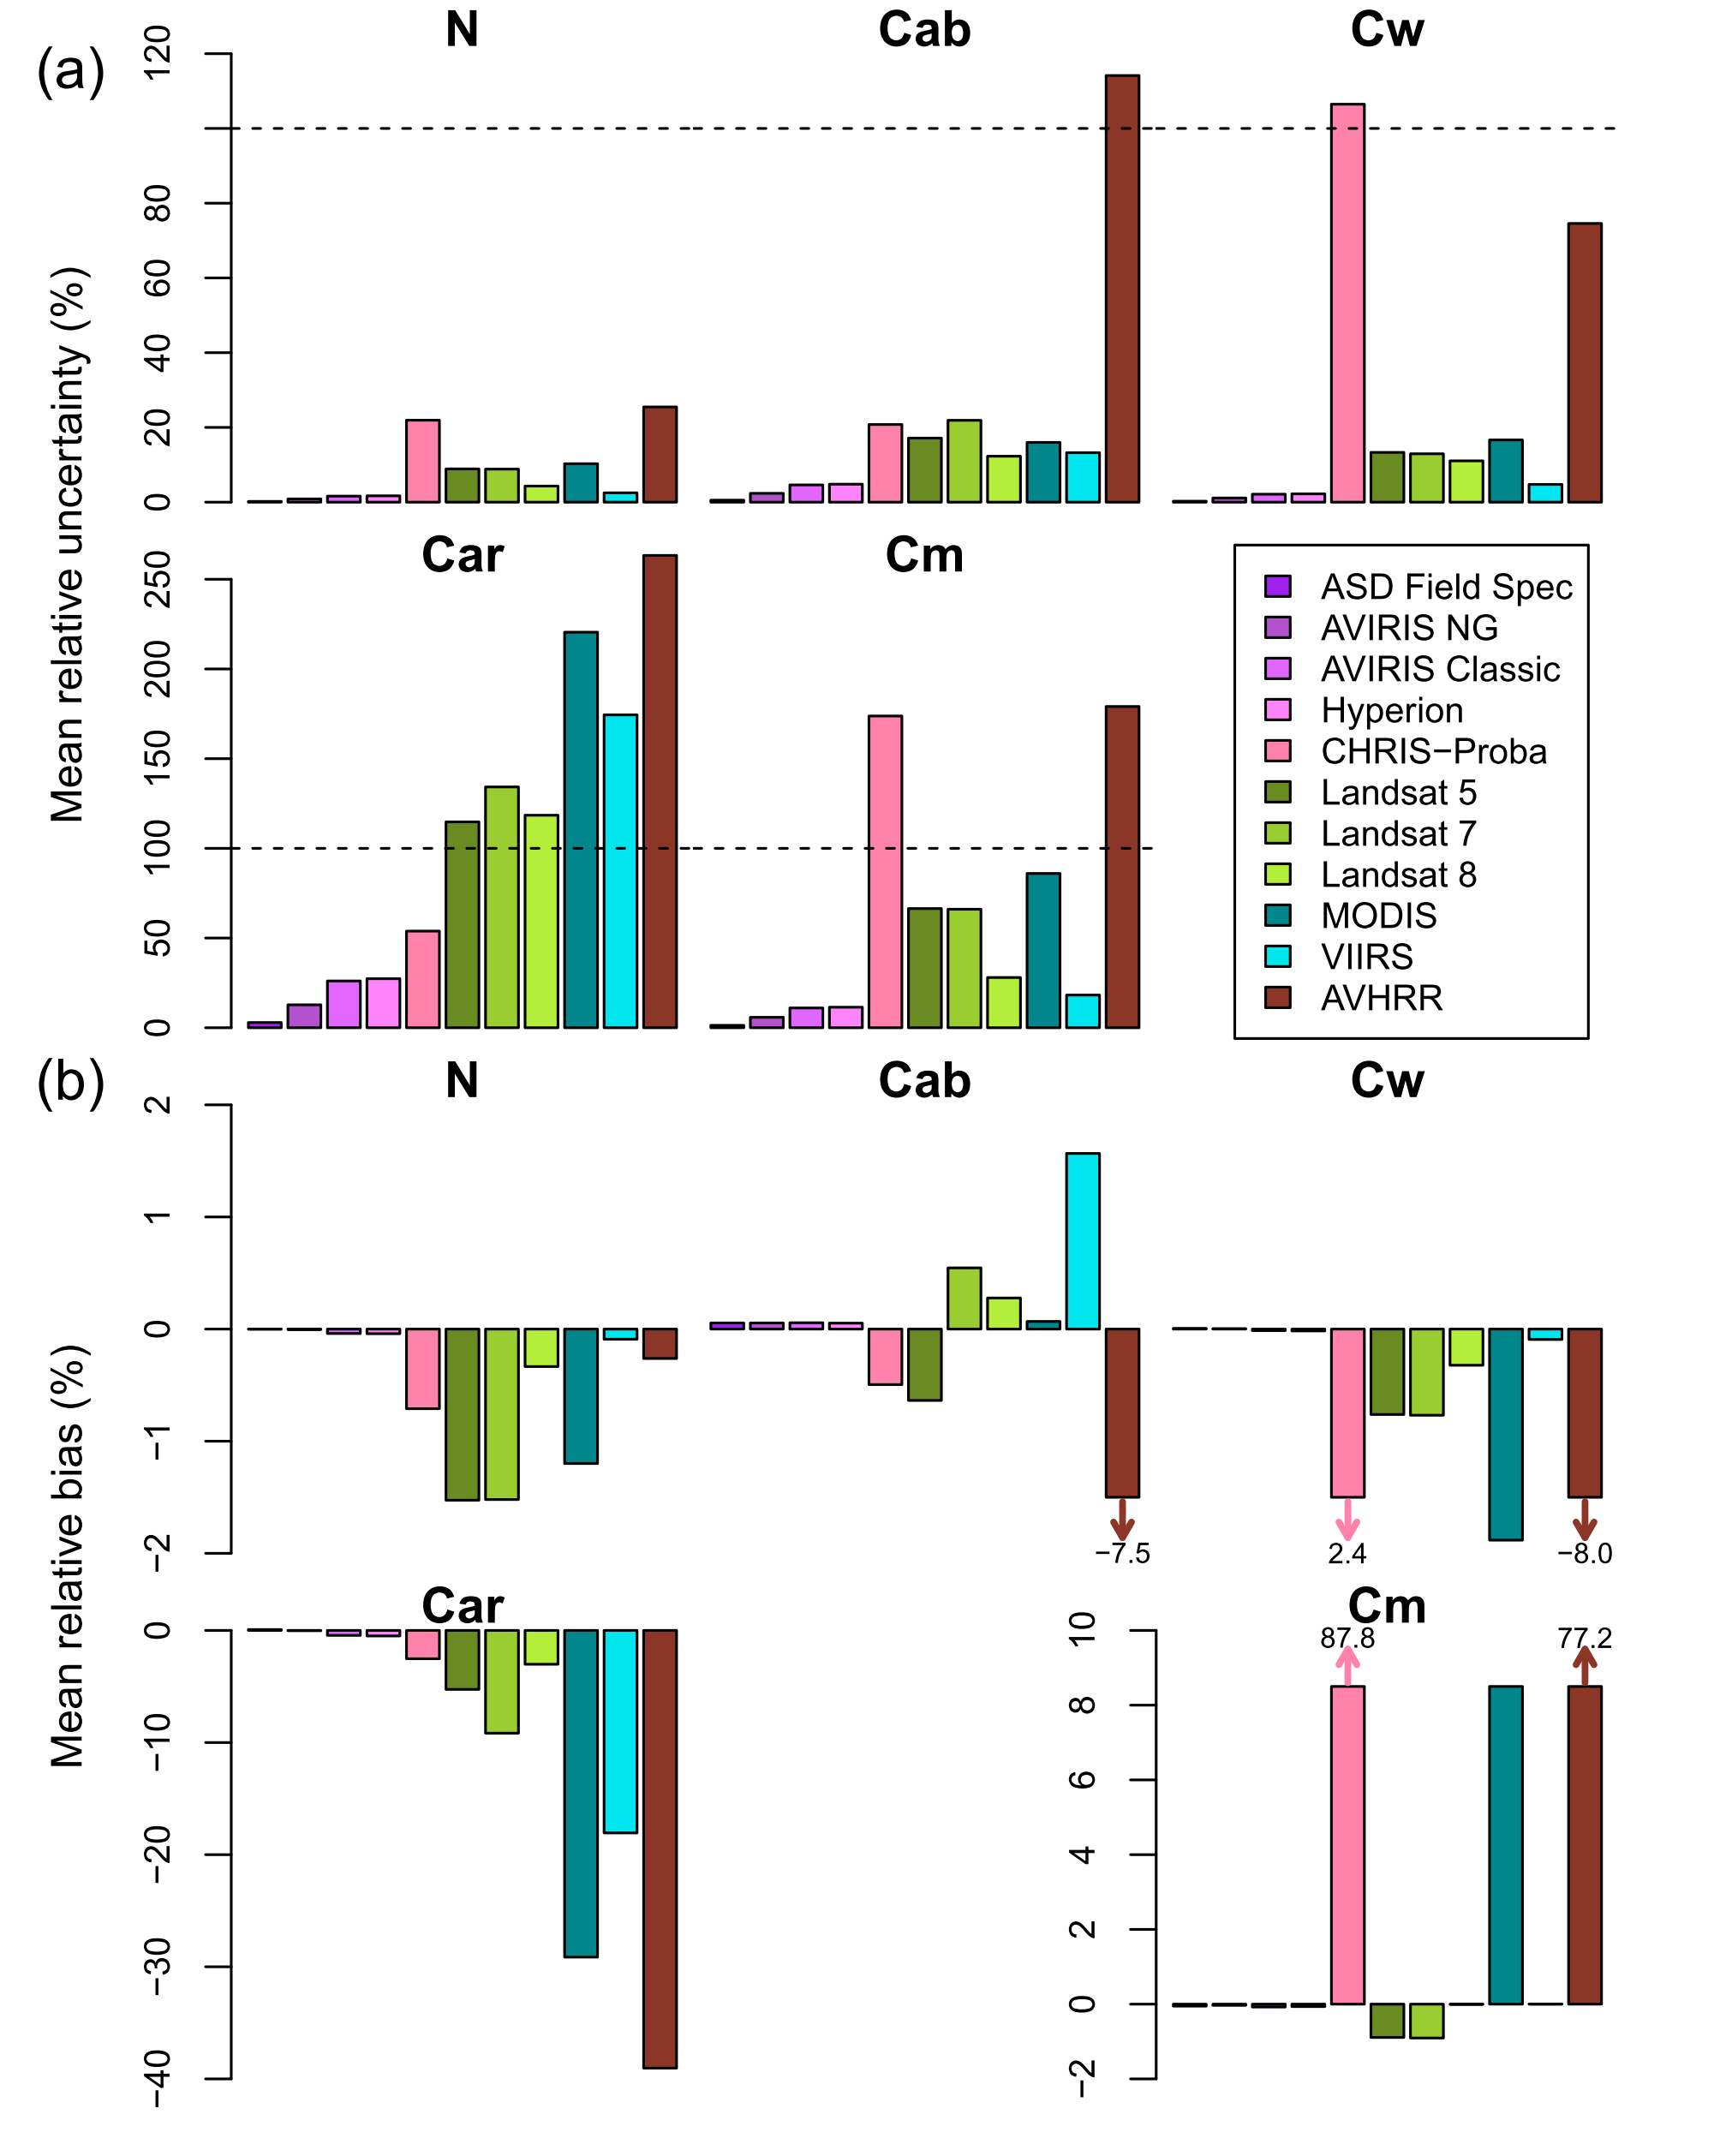
\includegraphics[width=\textwidth]{2_rtm_inversion/figures/mean_error.png}
  \caption{%
    Mean uncertainty (a) and relative bias (b) (as defined in section 2.3) of inversion estimates for each parameter and simulated sensor.
    Sensors are arranged along the x-axis in approximate order of increasing spectral resolution.
  }\label{fig:pecanrtm-sensorerror}
\end{figure}

Across all of the selected sensors, the highest PROSPECT 5 parameter inversion uncertainty and bias were observed for Car (Figure~\ref{fig:pecanrtm-sensorerror}, Table~\ref{tab:pecanrtm-sensorerror}).
This can readily be explained by the Car specific absorption feature, which is both extremely narrow and overlaps substantially with that of Cab (not shown).% (Figure S1). %TODO: Figure
On the other extreme, the most accurate and least uncertain retrieved parameter was N, which is related to the reflectivity of the leaf across the entire spectrum (Figure~\ref{fig:pecanrtm-sensorerror}, Table~\ref{tab:pecanrtm-sensorerror}).%, Figure S1). %TODO: Figure
Despite relatively narrow absorption features, most simulated sensors were able to retrieve Cab with reasonably good accuracy, which is not surprising given the long history of monitoring vegetation pigmentation using various platforms.
Similarly, all sensors except CHRIS-Proba and AVHRR retrieved Cw with low uncertainty and bias, reflecting the wide and strong absorption features of water in the NIR and SWIR (Figure~\ref{fig:pecanrtm-sensorerror}, Table~\ref{tab:pecanrtm-sensorerror}).%, Figure S1). %TODO: Figure
The failure of CHRIS-Proba to retrieve Cw can be attributed to its inability to measure in this spectral range.% (Figure S4). %TODO: Figure
The retrieval accuracy for Cm was much more sensor dependent, with good performance among the simulated hyperspectral sensors, VIIRS, and Landsat 8, followed by lower performance for simulated Landsat 5 and 7 and MODIS, and a poor result for the simulated Chris-PROBA and AVHRR data (Figure~\ref{fig:pecanrtm-sensorerror}, Table~\ref{fig:pecanrtm-sensorerror}).
Although the specific absorption feature for Cm is very wide, the sensitivity of reflectance to Cm values is much lower than for other parameters and almost the entire feature can be masked or confounded by Cw (Figure S1). %TODO: Figure
This suggests that Cm is very dependent on precise locations of certain bands and therefore explains the differences in the estimate accuracy of apparently similar sensors like Landsat 5, 7, and 8 (Table~\ref{tab:pecanrtm-sensors})%, Figure S4). %TODO: Figure
More generally, the importance of precise band widths and locations is evidenced by the noticeably better performance of Landsat 8 compared to Landsat 5 and 7 for certain parameters (Figure~\ref{fig:pecanrtm-sensorerror}, Table~\ref{fig:pecanrtm-sensorerror}) despite the subtle differences in the sensors’ respective bandwidths (Table~\ref{tab:pecanrtm-sensors})%, Figure S4). %TODO: Figure

\subsubsection{Parameter uncertainty and covariance}

\begin{figure}
  \centering
  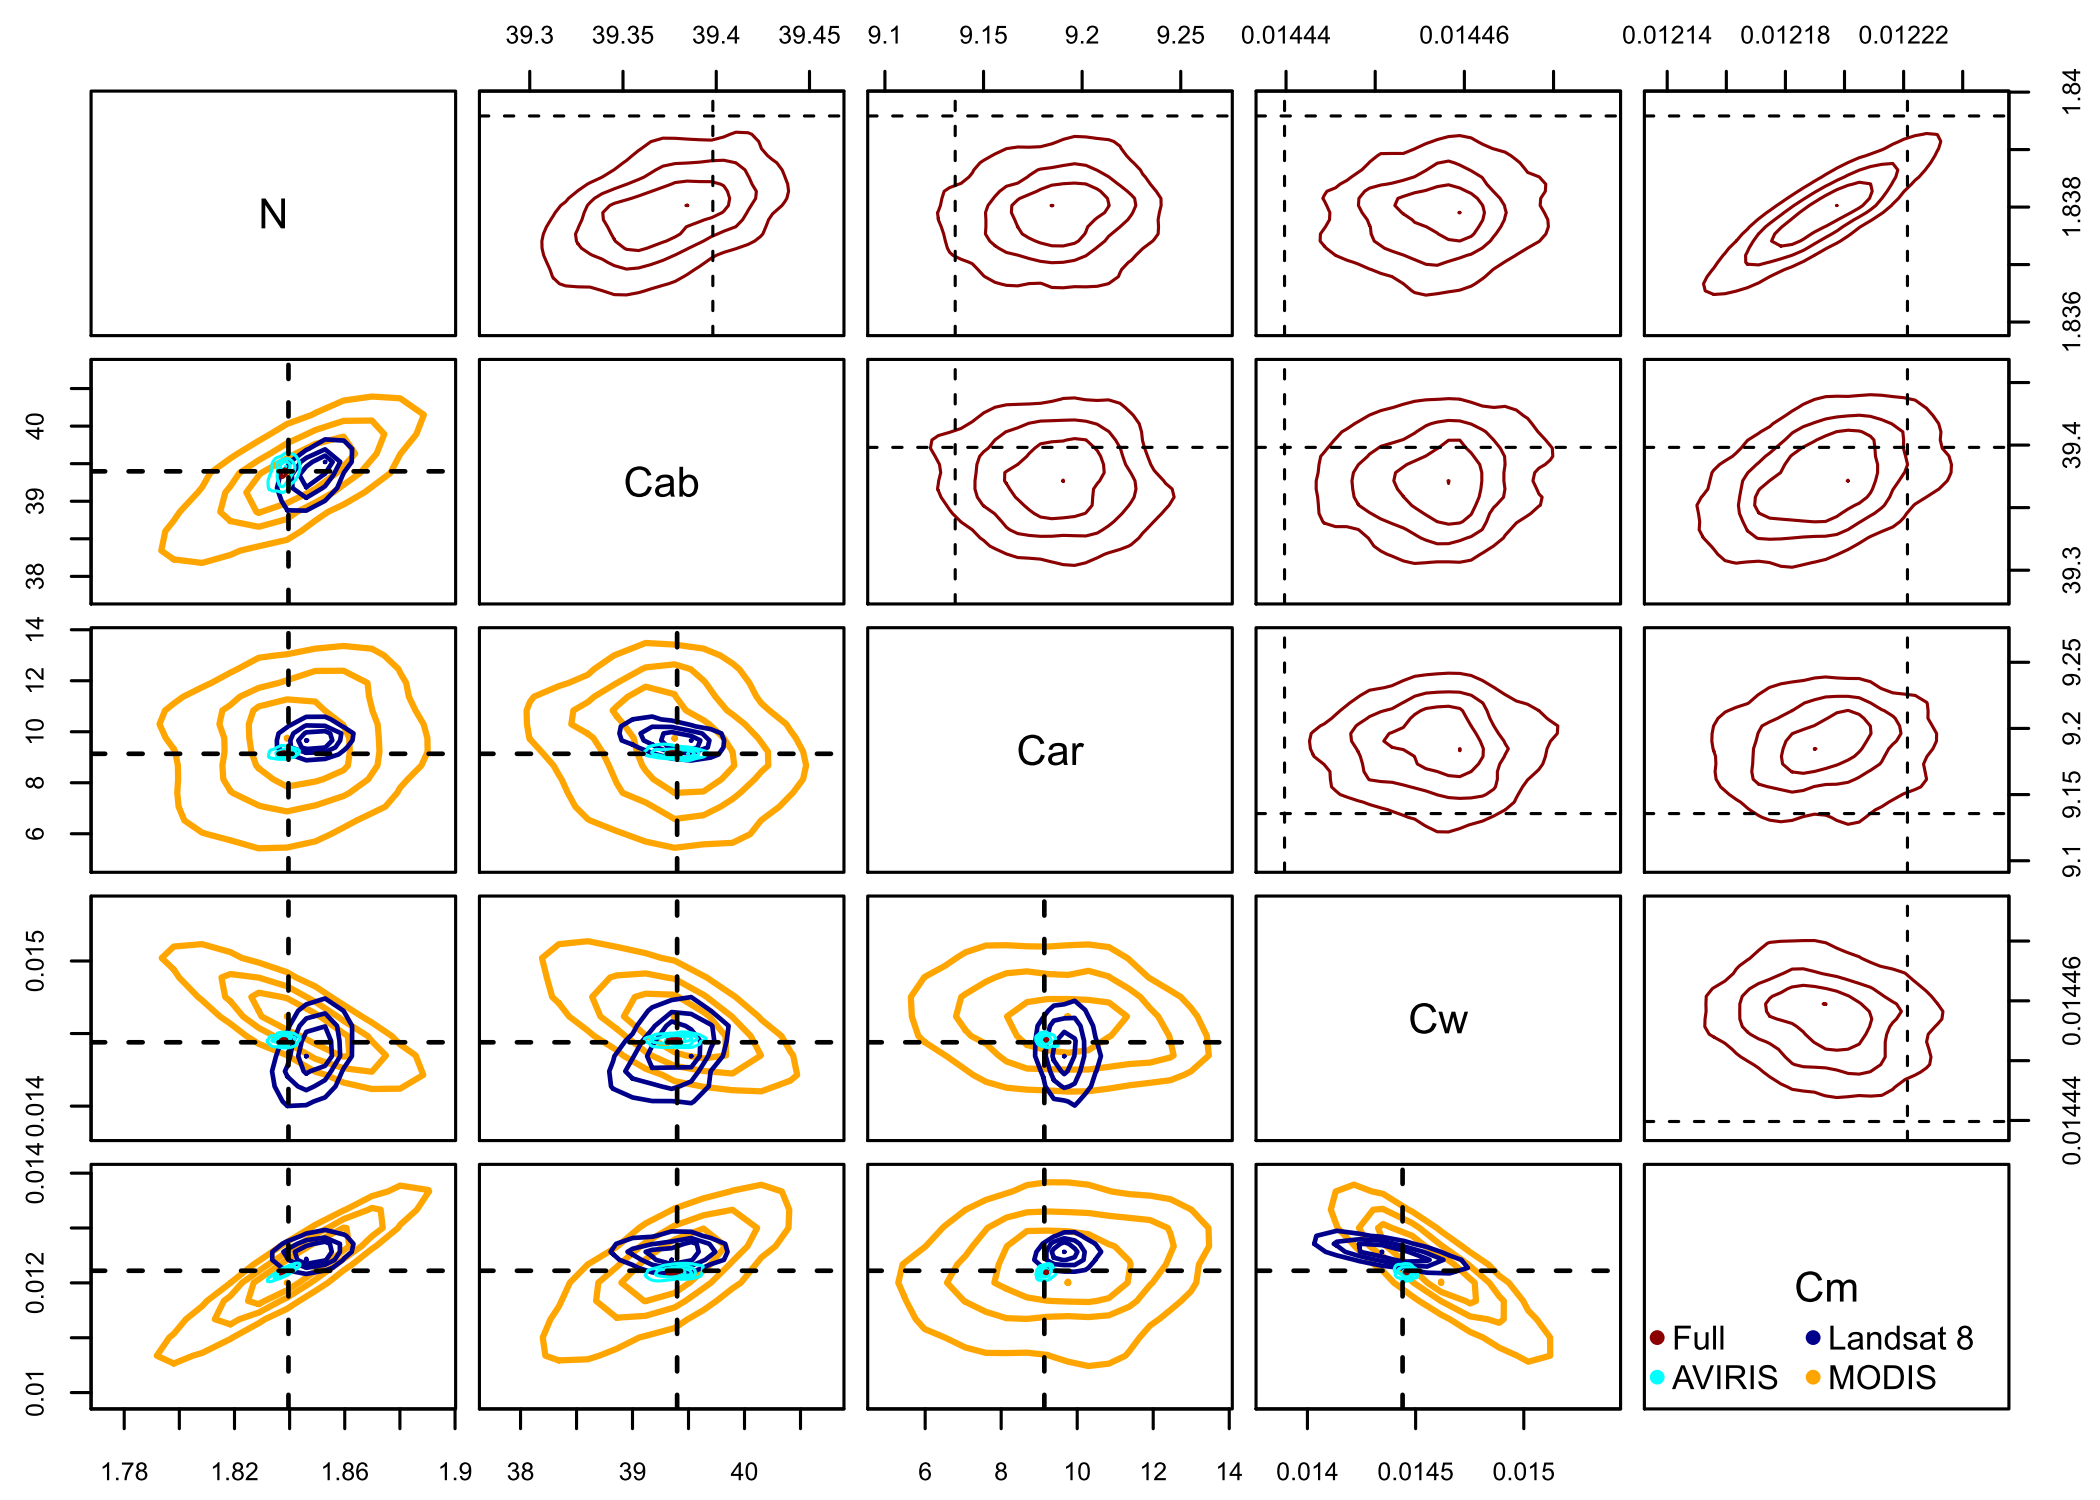
\includegraphics[width=\textwidth]{2_rtm_inversion/figures/joint_posterior.png}
  \caption{%
    Example joint probability distribution for parameter inversion estimates of simulated spectra using the full spectra (red; top panels) and the relative spectral response functions of AVIRIS NG (cyan), Landsat 8 (dark blue), and MODIS (orange). 
    Dotted lines indicate true parameter values. Note that the axis range of the top panels is substantially smaller than that of the bottom panels.
  }\label{fig:pecanrtm-jointpost}
\end{figure}

Figure~\ref{fig:pecanrtm-jointpost} shows an example of processed inversion output based on the high spectral resolution field spectrometer data and the spectral response functions of AVIRIS NG, Landsat 8, and MODIS\@.
All four plots are simulated from a single set of parameters, so differences in results are caused only by variations in spectral measurement characteristics.% (Figure S4). %TODO: Figure
Out of these four sensors, the uncertainties increase with approximately decreasing spectral resolution, with lowest uncertainties in the full spectra, second-lowest for AVIRIS NG, second highest for Landsat 8, and highest for MODIS\@. %TODO: Figure
The shapes of parameter covariances are distinctly different between these sensors, reflecting differences in the ability of the inversion to distinguish between parameters based on the available information.
Across all four sensors, we observe strong positive covariance between N and Cm, since these parameters influence wide regions of the reflectance spectrum in opposite ways.% (Figure S1). %TODO: Figure
Similarly, we also observe a positive covariance between N and Cab, although the strength of this covariance is not equal across sensors.
The remaining covariances are mostly specific to MODIS, whose band configuration increases the overlap between the associated parameters.% (Figure S4). %TODO: Figure

We find that inversion estimates for the field spectra are occasionally falsely overconfident.
For instance, the true value of N and Cw is outside the 95\% confidence limit of their estimated joint probability distribution at full, field spectrometer resolution.
That being said, this is less of an issue for the other sensors, where the joint probability distribution encompasses the true value.
This suggests that spectral resolution below 5 nm may not provide additional information content, particularly for the broad absorption features within leaves, because of the strong autocorrelation between adjacent wavelengths.
More importantly, although the joint posterior probability distributions from Landsat 8 and MODIS appear wide, the resulting parameter values are constrained by an order of magnitude or more compared to the priors.
